% REV00 Fri 26 Mar 2021 17:51:51 WIB
% START Fri 26 Mar 2021 17:51:51 WIB

\chapter{THE R. WILFER FAMILY}


Reginald Wilfer is a name with rather a grand sound, suggesting on
first acquaintance brasses in country churches, scrolls in stained-glass
windows, and generally the De Wilfers who came over with the Conqueror.
For, it is a remarkable fact in genealogy that no De Any ones ever came
over with Anybody else.

But, the Reginald Wilfer family were of such commonplace extraction and
pursuits that their forefathers had for generations modestly subsisted
on the Docks, the Excise Office, and the Custom House, and the existing
R. Wilfer was a poor clerk. So poor a clerk, though having a limited
salary and an unlimited family, that he had never yet attained the
modest object of his ambition: which was, to wear a complete new suit
of clothes, hat and boots included, at one time. His black hat was brown
before he could afford a coat, his pantaloons were white at the seams
and knees before he could buy a pair of boots, his boots had worn out
before he could treat himself to new pantaloons, and, by the time he
worked round to the hat again, that shining modern article roofed-in an
ancient ruin of various periods.

If the conventional Cherub could ever grow up and be clothed, he might
be photographed as a portrait of Wilfer. His chubby, smooth, innocent
appearance was a reason for his being always treated with condescension
when he was not put down. A stranger entering his own poor house at
about ten o’clock P.M. might have been surprised to find him sitting up
to supper. So boyish was he in his curves and proportions, that his
old schoolmaster meeting him in Cheapside, might have been unable to
withstand the temptation of caning him on the spot. In short, he was
the conventional cherub, after the supposititious shoot just mentioned,
rather grey, with signs of care on his expression, and in decidedly
insolvent circumstances.

He was shy, and unwilling to own to the name of Reginald, as being too
aspiring and self-assertive a name. In his signature he used only the
initial R., and imparted what it really stood for, to none but chosen
friends, under the seal of confidence. Out of this, the facetious habit
had arisen in the neighbourhood surrounding Mincing Lane of making
christian names for him of adjectives and participles beginning with R.
Some of these were more or less appropriate: as Rusty, Retiring, Ruddy,
Round, Ripe, Ridiculous, Ruminative; others, derived their point from
their want of application: as Raging, Rattling, Roaring, Raffish. But,
his popular name was Rumty, which in a moment of inspiration had been
bestowed upon him by a gentleman of convivial habits connected with the
drug-markets, as the beginning of a social chorus, his leading part in
the execution of which had led this gentleman to the Temple of Fame, and
of which the whole expressive burden ran:

     ‘Rumty iddity, row dow dow,
     Sing toodlely, teedlely, bow wow wow.’

Thus he was constantly addressed, even in minor notes on business, as
‘Dear Rumty’; in answer to which, he sedately signed himself, ‘Yours
truly, R. Wilfer.’

He was clerk in the drug-house of Chicksey, Veneering, and Stobbles.
Chicksey and Stobbles, his former masters, had both become absorbed in
Veneering, once their traveller or commission agent: who had signalized
his accession to supreme power by bringing into the business a quantity
of plate-glass window and French-polished mahogany partition, and a
gleaming and enormous doorplate.

R. Wilfer locked up his desk one evening, and, putting his bunch of keys
in his pocket much as if it were his peg-top, made for home. His home
was in the Holloway region north of London, and then divided from it by
fields and trees. Between Battle Bridge and that part of the Holloway
district in which he dwelt, was a tract of suburban Sahara, where tiles
and bricks were burnt, bones were boiled, carpets were beat, rubbish was
shot, dogs were fought, and dust was heaped by contractors. Skirting
the border of this desert, by the way he took, when the light of its
kiln-fires made lurid smears on the fog, R. Wilfer sighed and shook his
head.

‘Ah me!’ said he, ‘what might have been is not what is!’

With which commentary on human life, indicating an experience of it
not exclusively his own, he made the best of his way to the end of his
journey.

Mrs Wilfer was, of course, a tall woman and an angular. Her lord being
cherubic, she was necessarily majestic, according to the principle which
matrimonially unites contrasts. She was much given to tying up her head
in a pocket-handkerchief, knotted under the chin. This head-gear, in
conjunction with a pair of gloves worn within doors, she seemed to
consider as at once a kind of armour against misfortune (invariably
assuming it when in low spirits or difficulties), and as a species of
full dress. It was therefore with some sinking of the spirit that her
husband beheld her thus heroically attired, putting down her candle in
the little hall, and coming down the doorsteps through the little front
court to open the gate for him.

Something had gone wrong with the house-door, for R. Wilfer stopped on
the steps, staring at it, and cried:

‘Hal-loa?’

‘Yes,’ said Mrs Wilfer, ‘the man came himself with a pair of pincers,
and took it off, and took it away. He said that as he had no expectation
of ever being paid for it, and as he had an order for another LADIES’
SCHOOL door-plate, it was better (burnished up) for the interests of all
parties.’

‘Perhaps it was, my dear; what do you think?’

‘You are master here, R. W.,’ returned his wife. ‘It is as you think;
not as I do. Perhaps it might have been better if the man had taken the
door too?’

‘My dear, we couldn’t have done without the door.’

‘Couldn’t we?’

‘Why, my dear! Could we?’

‘It is as you think, R. W.; not as I do.’ With those submissive words,
the dutiful wife preceded him down a few stairs to a little basement
front room, half kitchen, half parlour, where a girl of about nineteen,
with an exceedingly pretty figure and face, but with an impatient and
petulant expression both in her face and in her shoulders (which in
her sex and at her age are very expressive of discontent), sat playing
draughts with a younger girl, who was the youngest of the House of
Wilfer. Not to encumber this page by telling off the Wilfers in detail
and casting them up in the gross, it is enough for the present that the
rest were what is called ‘out in the world,’ in various ways, and that
they were Many. So many, that when one of his dutiful children called in
to see him, R. Wilfer generally seemed to say to himself, after a little
mental arithmetic, ‘Oh! here’s another of ‘em!’ before adding aloud,
‘How de do, John,’ or Susan, as the case might be.

‘Well Piggywiggies,’ said R. W., ‘how de do to-night? What I was
thinking of, my dear,’ to Mrs Wilfer already seated in a corner with
folded gloves, ‘was, that as we have let our first floor so well, and as
we have now no place in which you could teach pupils even if pupils--’

‘The milkman said he knew of two young ladies of the highest
respectability who were in search of a suitable establishment, and he
took a card,’ interposed Mrs Wilfer, with severe monotony, as if she
were reading an Act of Parliament aloud. ‘Tell your father whether it
was last Monday, Bella.’

‘But we never heard any more of it, ma,’ said Bella, the elder girl.

‘In addition to which, my dear,’ her husband urged, ‘if you have no
place to put two young persons into--’

‘Pardon me,’ Mrs Wilfer again interposed; ‘they were not young persons.
Two young ladies of the highest respectability. Tell your father, Bella,
whether the milkman said so.’

‘My dear, it is the same thing.’

‘No it is not,’ said Mrs Wilfer, with the same impressive monotony.
‘Pardon me!’

‘I mean, my dear, it is the same thing as to space. As to space. If you
have no space in which to put two youthful fellow-creatures, however
eminently respectable, which I do not doubt, where are those youthful
fellow-creatures to be accommodated? I carry it no further than that.
And solely looking at it,’ said her husband, making the stipulation at
once in a conciliatory, complimentary, and argumentative tone--‘as I am
sure you will agree, my love--from a fellow-creature point of view, my
dear.’

‘I have nothing more to say,’ returned Mrs Wilfer, with a meek
renunciatory action of her gloves. ‘It is as you think, R. W.; not as I
do.’

Here, the huffing of Miss Bella and the loss of three of her men at a
swoop, aggravated by the coronation of an opponent, led to that young
lady’s jerking the draught-board and pieces off the table: which her
sister went down on her knees to pick up.

‘Poor Bella!’ said Mrs Wilfer.

‘And poor Lavinia, perhaps, my dear?’ suggested R. W.

‘Pardon me,’ said Mrs Wilfer, ‘no!’

It was one of the worthy woman’s specialities that she had an amazing
power of gratifying her splenetic or worldly-minded humours by extolling
her own family: which she thus proceeded, in the present case, to do.

‘No, R. W. Lavinia has not known the trial that Bella has known. The
trial that your daughter Bella has undergone, is, perhaps, without
a parallel, and has been borne, I will say, Nobly. When you see your
daughter Bella in her black dress, which she alone of all the family
wears, and when you remember the circumstances which have led to
her wearing it, and when you know how those circumstances have been
sustained, then, R. W., lay your head upon your pillow and say, “Poor
Lavinia!”’

Here, Miss Lavinia, from her kneeling situation under the table, put in
that she didn’t want to be ‘poored by pa’, or anybody else.

‘I am sure you do not, my dear,’ returned her mother, ‘for you have a
fine brave spirit. And your sister Cecilia has a fine brave spirit
of another kind, a spirit of pure devotion, a beau-ti-ful spirit! The
self-sacrifice of Cecilia reveals a pure and womanly character, very
seldom equalled, never surpassed. I have now in my pocket a letter from
your sister Cecilia, received this morning--received three months after
her marriage, poor child!--in which she tells me that her husband must
unexpectedly shelter under their roof his reduced aunt. “But I will be
true to him, mamma,” she touchingly writes, “I will not leave him, I
must not forget that he is my husband. Let his aunt come!” If this is
not pathetic, if this is not woman’s devotion--!’ The good lady waved
her gloves in a sense of the impossibility of saying more, and tied the
pocket-handkerchief over her head in a tighter knot under her chin.

Bella, who was now seated on the rug to warm herself, with her brown
eyes on the fire and a handful of her brown curls in her mouth, laughed
at this, and then pouted and half cried.

‘I am sure,’ said she, ‘though you have no feeling for me, pa, I am one
of the most unfortunate girls that ever lived. You know how poor we are’
(it is probable he did, having some reason to know it!), ‘and what a
glimpse of wealth I had, and how it melted away, and how I am here in
this ridiculous mourning--which I hate!--a kind of a widow who never was
married. And yet you don’t feel for me.--Yes you do, yes you do.’

This abrupt change was occasioned by her father’s face. She stopped
to pull him down from his chair in an attitude highly favourable to
strangulation, and to give him a kiss and a pat or two on the cheek.

‘But you ought to feel for me, you know, pa.’

‘My dear, I do.’

‘Yes, and I say you ought to. If they had only left me alone and told
me nothing about it, it would have mattered much less. But that nasty Mr
Lightwood feels it his duty, as he says, to write and tell me what is in
reserve for me, and then I am obliged to get rid of George Sampson.’

Here, Lavinia, rising to the surface with the last draughtman rescued,
interposed, ‘You never cared for George Sampson, Bella.’

‘And did I say I did, miss?’ Then, pouting again, with the curls in her
mouth; ‘George Sampson was very fond of me, and admired me very much,
and put up with everything I did to him.’

‘You were rude enough to him,’ Lavinia again interposed.

‘And did I say I wasn’t, miss? I am not setting up to be sentimental
about George Sampson. I only say George Sampson was better than
nothing.’

‘You didn’t show him that you thought even that,’ Lavinia again
interposed.

‘You are a chit and a little idiot,’ returned Bella, ‘or you wouldn’t
make such a dolly speech. What did you expect me to do? Wait till you
are a woman, and don’t talk about what you don’t understand. You only
show your ignorance!’ Then, whimpering again, and at intervals biting
the curls, and stopping to look how much was bitten off, ‘It’s a shame!
There never was such a hard case! I shouldn’t care so much if it wasn’t
so ridiculous. It was ridiculous enough to have a stranger coming over
to marry me, whether he liked it or not. It was ridiculous enough to
know what an embarrassing meeting it would be, and how we never
could pretend to have an inclination of our own, either of us. It was
ridiculous enough to know I shouldn’t like him--how COULD I like him,
left to him in a will, like a dozen of spoons, with everything cut and
dried beforehand, like orange chips. Talk of orange flowers indeed!
I declare again it’s a shame! Those ridiculous points would have been
smoothed away by the money, for I love money, and want money--want it
dreadfully. I hate to be poor, and we are degradingly poor, offensively
poor, miserably poor, beastly poor. But here I am, left with all the
ridiculous parts of the situation remaining, and, added to them all,
this ridiculous dress! And if the truth was known, when the Harmon
murder was all over the town, and people were speculating on its being
suicide, I dare say those impudent wretches at the clubs and places made
jokes about the miserable creature’s having preferred a watery grave to
me. It’s likely enough they took such liberties; I shouldn’t wonder! I
declare it’s a very hard case indeed, and I am a most unfortunate girl.
The idea of being a kind of a widow, and never having been married!
And the idea of being as poor as ever after all, and going into black,
besides, for a man I never saw, and should have hated--as far as HE was
concerned--if I had seen!’

The young lady’s lamentations were checked at this point by a knuckle,
knocking at the half-open door of the room. The knuckle had knocked two
or three times already, but had not been heard.

‘Who is it?’ said Mrs Wilfer, in her Act-of-Parliament manner. ‘Enter!’

A gentleman coming in, Miss Bella, with a short and sharp exclamation,
scrambled off the hearth-rug and massed the bitten curls together in
their right place on her neck.

‘The servant girl had her key in the door as I came up, and directed me
to this room, telling me I was expected. I am afraid I should have asked
her to announce me.’

‘Pardon me,’ returned Mrs Wilfer. ‘Not at all. Two of my daughters. R.
W., this is the gentleman who has taken your first-floor. He was so good
as to make an appointment for to-night, when you would be at home.’

A dark gentleman. Thirty at the utmost. An expressive, one might say
handsome, face. A very bad manner. In the last degree constrained,
reserved, diffident, troubled. His eyes were on Miss Bella for an
instant, and then looked at the ground as he addressed the master of the
house.

‘Seeing that I am quite satisfied, Mr Wilfer, with the rooms, and with
their situation, and with their price, I suppose a memorandum between us
of two or three lines, and a payment down, will bind the bargain? I wish
to send in furniture without delay.’

Two or three times during this short address, the cherub addressed had
made chubby motions towards a chair. The gentleman now took it, laying
a hesitating hand on a corner of the table, and with another hesitating
hand lifting the crown of his hat to his lips, and drawing it before his
mouth.

‘The gentleman, R. W.,’ said Mrs Wilfer, ‘proposes to take your
apartments by the quarter. A quarter’s notice on either side.’

‘Shall I mention, sir,’ insinuated the landlord, expecting it to be
received as a matter of course, ‘the form of a reference?’

‘I think,’ returned the gentleman, after a pause, ‘that a reference is
not necessary; neither, to say the truth, is it convenient, for I am
a stranger in London. I require no reference from you, and perhaps,
therefore, you will require none from me. That will be fair on both
sides. Indeed, I show the greater confidence of the two, for I will pay
in advance whatever you please, and I am going to trust my furniture
here. Whereas, if you were in embarrassed circumstances--this is merely
supposititious--’

Conscience causing R. Wilfer to colour, Mrs Wilfer, from a corner (she
always got into stately corners) came to the rescue with a deep-toned
‘Per-fectly.’

‘--Why then I--might lose it.’

‘Well!’ observed R. Wilfer, cheerfully, ‘money and goods are certainly
the best of references.’

‘Do you think they ARE the best, pa?’ asked Miss Bella, in a low voice,
and without looking over her shoulder as she warmed her foot on the
fender.

‘Among the best, my dear.’

‘I should have thought, myself, it was so easy to add the usual kind of
one,’ said Bella, with a toss of her curls.

The gentleman listened to her, with a face of marked attention, though
he neither looked up nor changed his attitude. He sat, still and silent,
until his future landlord accepted his proposals, and brought writing
materials to complete the business. He sat, still and silent, while the
landlord wrote.

When the agreement was ready in duplicate (the landlord having worked
at it like some cherubic scribe, in what is conventionally called a
doubtful, which means a not at all doubtful, Old Master), it was signed
by the contracting parties, Bella looking on as scornful witness. The
contracting parties were R. Wilfer, and John Rokesmith Esquire.

When it came to Bella’s turn to sign her name, Mr Rokesmith, who was
standing, as he had sat, with a hesitating hand upon the table, looked
at her stealthily, but narrowly. He looked at the pretty figure bending
down over the paper and saying, ‘Where am I to go, pa? Here, in this
corner?’ He looked at the beautiful brown hair, shading the coquettish
face; he looked at the free dash of the signature, which was a bold one
for a woman’s; and then they looked at one another.

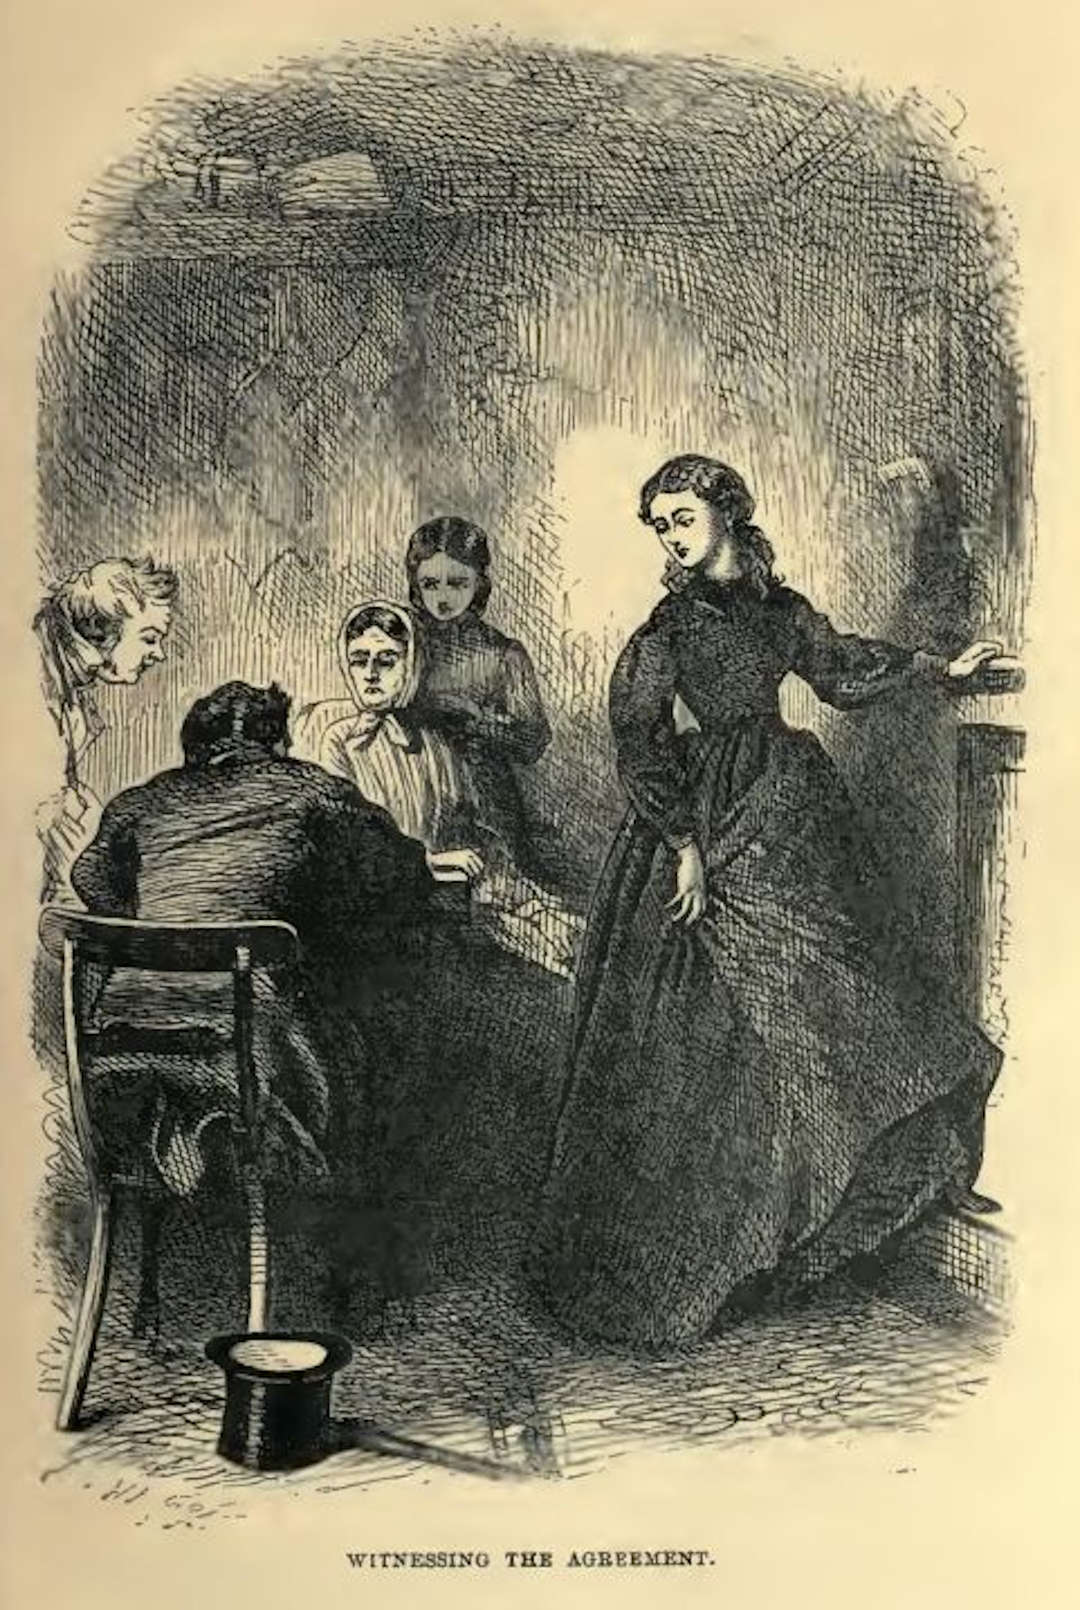
\includegraphics[scale=2.3]{01-04-01}

‘Much obliged to you, Miss Wilfer.’

‘Obliged?’

‘I have given you so much trouble.’

‘Signing my name? Yes, certainly. But I am your landlord’s daughter,
sir.’

As there was nothing more to do but pay eight sovereigns in earnest of
the bargain, pocket the agreement, appoint a time for the arrival of his
furniture and himself, and go, Mr Rokesmith did that as awkwardly as it
might be done, and was escorted by his landlord to the outer air. When
R. Wilfer returned, candlestick in hand, to the bosom of his family, he
found the bosom agitated.

‘Pa,’ said Bella, ‘we have got a Murderer for a tenant.’

‘Pa,’ said Lavinia, ‘we have got a Robber.’

‘To see him unable for his life to look anybody in the face!’ said
Bella. ‘There never was such an exhibition.’

‘My dears,’ said their father, ‘he is a diffident gentleman, and I
should say particularly so in the society of girls of your age.’

‘Nonsense, our age!’ cried Bella, impatiently. ‘What’s that got to do
with him?’

‘Besides, we are not of the same age:--which age?’ demanded Lavinia.

‘Never YOU mind, Lavvy,’ retorted Bella; ‘you wait till you are of an
age to ask such questions. Pa, mark my words! Between Mr Rokesmith and
me, there is a natural antipathy and a deep distrust; and something will
come of it!’

‘My dear, and girls,’ said the cherub-patriarch, ‘between Mr Rokesmith
and me, there is a matter of eight sovereigns, and something for supper
shall come of it, if you’ll agree upon the article.’

This was a neat and happy turn to give the subject, treats being rare in
the Wilfer household, where a monotonous appearance of Dutch-cheese at
ten o’clock in the evening had been rather frequently commented on by
the dimpled shoulders of Miss Bella. Indeed, the modest Dutchman himself
seemed conscious of his want of variety, and generally came before the
family in a state of apologetic perspiration. After some discussion on
the relative merits of veal-cutlet, sweetbread, and lobster, a decision
was pronounced in favour of veal-cutlet. Mrs Wilfer then solemnly
divested herself of her handkerchief and gloves, as a preliminary
sacrifice to preparing the frying-pan, and R. W. himself went out
to purchase the viand. He soon returned, bearing the same in a fresh
cabbage-leaf, where it coyly embraced a rasher of ham. Melodious sounds
were not long in rising from the frying-pan on the fire, or in seeming,
as the firelight danced in the mellow halls of a couple of full bottles
on the table, to play appropriate dance-music.

The cloth was laid by Lavvy. Bella, as the acknowledged ornament of the
family, employed both her hands in giving her hair an additional
wave while sitting in the easiest chair, and occasionally threw in a
direction touching the supper: as, ‘Very brown, ma;’ or, to her sister,
‘Put the saltcellar straight, miss, and don’t be a dowdy little puss.’

Meantime her father, chinking Mr Rokesmith’s gold as he sat expectant
between his knife and fork, remarked that six of those sovereigns came
just in time for their landlord, and stood them in a little pile on the
white tablecloth to look at.

‘I hate our landlord!’ said Bella.

But, observing a fall in her father’s face, she went and sat down by him
at the table, and began touching up his hair with the handle of a fork.
It was one of the girl’s spoilt ways to be always arranging the family’s
hair--perhaps because her own was so pretty, and occupied so much of her
attention.

‘You deserve to have a house of your own; don’t you, poor pa?’

‘I don’t deserve it better than another, my dear.’

‘At any rate I, for one, want it more than another,’ said Bella, holding
him by the chin, as she stuck his flaxen hair on end, ‘and I grudge
this money going to the Monster that swallows up so much, when we all
want--Everything. And if you say (as you want to say; I know you want
to say so, pa) “that’s neither reasonable nor honest, Bella,” then I
answer, “Maybe not, pa--very likely--but it’s one of the consequences
of being poor, and of thoroughly hating and detesting to be poor, and
that’s my case.” Now, you look lovely, pa; why don’t you always wear
your hair like that? And here’s the cutlet! If it isn’t very brown, ma,
I can’t eat it, and must have a bit put back to be done expressly.’

However, as it was brown, even to Bella’s taste, the young lady
graciously partook of it without reconsignment to the frying-pan, and
also, in due course, of the contents of the two bottles: whereof
one held Scotch ale and the other rum. The latter perfume, with
the fostering aid of boiling water and lemon-peel, diffused itself
throughout the room, and became so highly concentrated around the warm
fireside, that the wind passing over the house roof must have rushed off
charged with a delicious whiff of it, after buzzing like a great bee at
that particular chimneypot.

‘Pa,’ said Bella, sipping the fragrant mixture and warming her favourite
ankle; ‘when old Mr Harmon made such a fool of me (not to mention
himself, as he is dead), what do you suppose he did it for?’

‘Impossible to say, my dear. As I have told you time out of number since
his will was brought to light, I doubt if I ever exchanged a hundred
words with the old gentleman. If it was his whim to surprise us, his
whim succeeded. For he certainly did it.’

‘And I was stamping my foot and screaming, when he first took notice of
me; was I?’ said Bella, contemplating the ankle before mentioned.

‘You were stamping your little foot, my dear, and screaming with your
little voice, and laying into me with your little bonnet, which you
had snatched off for the purpose,’ returned her father, as if the
remembrance gave a relish to the rum; ‘you were doing this one Sunday
morning when I took you out, because I didn’t go the exact way you
wanted, when the old gentleman, sitting on a seat near, said, “That’s a
nice girl; that’s a VERY nice girl; a promising girl!” And so you were,
my dear.’

‘And then he asked my name, did he, pa?’

‘Then he asked your name, my dear, and mine; and on other Sunday
mornings, when we walked his way, we saw him again, and--and really
that’s all.’

As that was all the rum and water too, or, in other words, as R. W.
delicately signified that his glass was empty, by throwing back his head
and standing the glass upside down on his nose and upper lip, it might
have been charitable in Mrs Wilfer to suggest replenishment. But that
heroine briefly suggesting ‘Bedtime’ instead, the bottles were put away,
and the family retired; she cherubically escorted, like some severe
saint in a painting, or merely human matron allegorically treated.

‘And by this time to-morrow,’ said Lavinia when the two girls were alone
in their room, ‘we shall have Mr Rokesmith here, and shall be expecting
to have our throats cut.’

‘You needn’t stand between me and the candle for all that,’ retorted
Bella. ‘This is another of the consequences of being poor! The idea of a
girl with a really fine head of hair, having to do it by one flat candle
and a few inches of looking-glass!’

‘You caught George Sampson with it, Bella, bad as your means of dressing
it are.’

‘You low little thing. Caught George Sampson with it! Don’t talk about
catching people, miss, till your own time for catching--as you call
it--comes.’

‘Perhaps it has come,’ muttered Lavvy, with a toss of her head.

‘What did you say?’ asked Bella, very sharply. ‘What did you say, miss?’

Lavvy declining equally to repeat or to explain, Bella gradually lapsed
over her hair-dressing into a soliloquy on the miseries of being poor,
as exemplified in having nothing to put on, nothing to go out in,
nothing to dress by, only a nasty box to dress at instead of a
commodious dressing-table, and being obliged to take in suspicious
lodgers. On the last grievance as her climax, she laid great stress--and
might have laid greater, had she known that if Mr Julius Handford had a
twin brother upon earth, Mr John Rokesmith was the man.


